\section{主实验：layout control 如何提升极低预算下的鲁棒性}

本章的结论是：MemOCR 在单跳和多跳长上下文问答中整体优于文本记忆基线，优势在 \texttt{memory budget} 缩小时最明显。关键原因来自 \texttt{layout control} 对证据位置的调度：直接影响答案的证据被放在更容易存活、更容易读取的位置。

\begin{importantbox}{本章主张}
主实验支持两层判断：第一，MemOCR 在有限记忆预算下保持了更高性能；第二，oracle analysis 显示同一条正确证据放入 \texttt{crucial area} 比放入 \texttt{detail area} 更能提升结果。这说明版面显著性本身参与了压缩鲁棒性的形成。
\end{importantbox}

\subsection{实验设置：上下文长度与记忆预算}

讲者在单跳和多跳长上下文问答任务上比较 MemOCR 与既有文本记忆方法。图表中的横向设置对应问答过程中模型总共看到的上下文规模，画面显示包括 $10K$、$30K$、$100K$ 三档；表格覆盖 HotpotQA、2Wiki、NQ、TriviaQA 等任务。这里的任务差异很重要：单跳问题通常只需定位一个事实，多跳问题需要把多条证据串起来，后者更容易暴露记忆压缩的断点。

纵向颜色或分组对应最终回答阶段用于存储记忆状态的 \texttt{memory budget}。换句话说，模型先完成记忆更新，再把最终形态的记忆以有限 token 预算塞回上下文中做问答。这个实验设计的核心检验对象是：长文被压成记忆后，关键证据还能不能在回答时被读出。

记忆预算可以写成：

$$
B = |\text{image tokens for visual memory}|
$$

其中：

\begin{itemize}
    \item $B$：最终回答阶段视觉记忆占用的 \texttt{image token} 数。
    \item $\text{image tokens for visual memory}$：用于表示视觉记忆图像的 token 集合，下文统一称为视觉记忆 token。
\end{itemize}

压缩鲁棒性可以用性能保持率表达：

$$
\text{Retention}(B) =
\frac{\text{Score}(B)}{\text{Score}_{\text{full context}}}
$$

其中：

\begin{itemize}
    \item $\text{Score}(B)$：给定记忆预算 $B$ 时的任务分数。
    \item $\text{Score}_{\text{full context}}$：完整上下文条件下的参考分数。
    \item $\text{Retention}(B)$：压缩后的能力保持率，越高表示在小预算下越稳。
\end{itemize}

\begin{figure}[H]
\centering
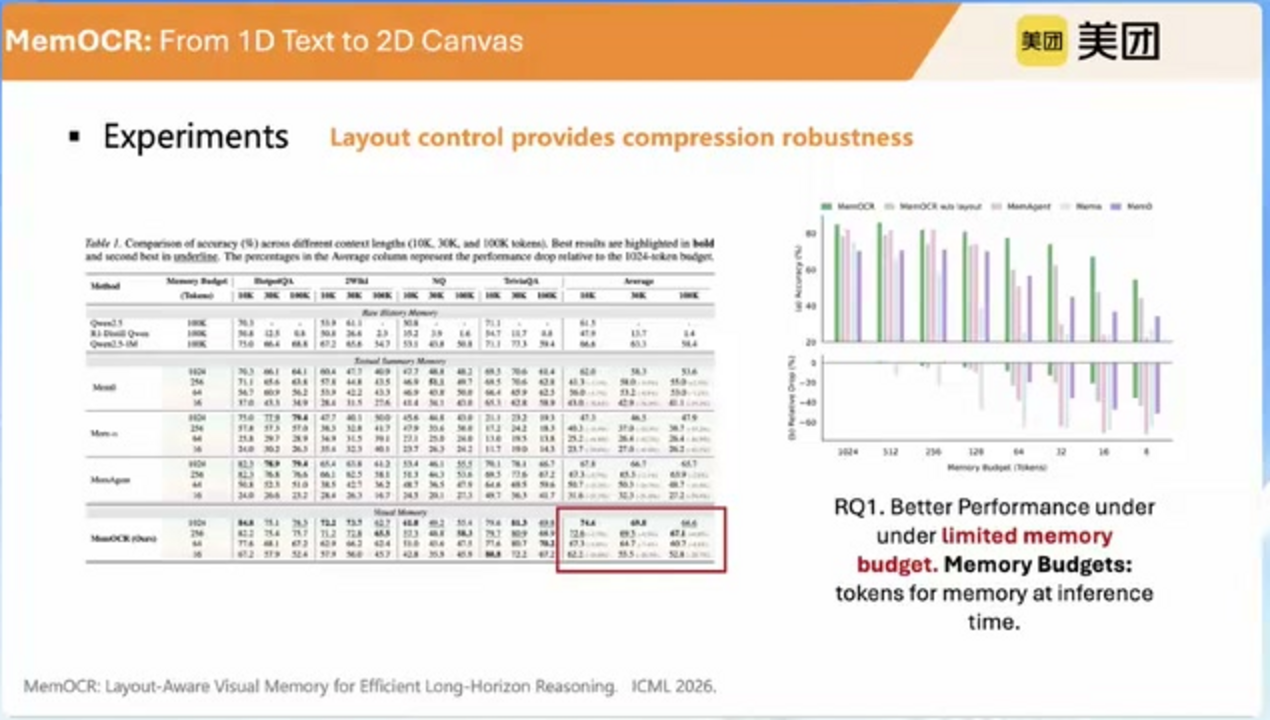
\includegraphics[width=0.86\linewidth,height=0.40\textheight,keepaspectratio]{figures/selected/fig05_memory_budget_results.png}
\caption{主实验结果：表格比较不同上下文长度和不同记忆预算下的准确率，右侧柱状图展示预算缩小时各方法的表现变化。读图重点是绿色 MemOCR 在小预算区域仍保持较高准确率。\protect\footnotemark}
\end{figure}
\footnotetext{视频画面时间区间：00:12:30--00:13:00。}

\subsection{主结果：极低预算下的性能保持}

实验的第一层发现是整体性能。讲者指出，MemOCR 在所有 memory-based agents 中展现出最好的整体表现。表格和柱状图也呈现出同一趋势：当预算从较大值逐步下降时，MemOCR 的下降幅度更小，尤其在极低预算端更明显。

更具体地说，字幕提到 MemOCR 可以仅用 $16$ 个视觉记忆 token 保留完整上下文能力的 $80\%+$；相对地，一些文本记忆基线在极端预算下平均性能会出现 $50\%--60\%$ 的下降。这个差异可以从第一性原理解释：文本摘要的 token 密度比较均匀，压缩时很难优先保护关键证据；视觉记忆可以把关键信息写在标题、中心区域或更醒目的块里，让低分辨率下仍有较高概率被读出。

\begin{knowledgebox}{怎样理解 $16$ 个视觉记忆 token}
$16$ 个视觉记忆 token 可以近似理解成一张被强烈压缩的记忆缩略图。此时模型很难稳定读取所有小字，因此真正能存活的往往是标题层级、显著区域和结构化标记。MemOCR 的优势正在于它训练模型把最该存活的信息放到这些位置。
\end{knowledgebox}

这个结果也提示一个工程含义：长程 agent 的记忆系统不能只问“压缩率有多高”，还要问“压缩后剩下的信息是不是答案需要的”。一个压缩器如果把所有内容等比例压小，看似公平，实际会让关键证据和背景噪声一起变得难读；一个 layout-aware 的压缩器会把有限预算优先分配给高价值证据。

\subsection{Oracle analysis：证据放在哪里更有价值}

主实验只能说明 MemOCR 表现更好，oracle analysis 进一步追问原因。讲者的设计是把 \texttt{ground truth}，也就是真正的正确答案或关键证据，直接注入视觉记忆，再比较注入位置的影响。两种设定分别是：把 oracle 信息放到 \texttt{crucial area}，例如更高层级的 headings 或更显著区域；把 oracle 信息放到 \texttt{detail area}，例如最低层级、接近普通正文的小字区域。

这个实验的结论很尖锐：当 oracle 信息被注入 \texttt{crucial area} 时，性能提升更明显，尤其在 $16$ 视觉记忆 token 预算这类低预算场景下提升最大；这种趋势同时出现在 multi-hop、single-hop、in-distribution 的 HotpotQA，以及 out-of-distribution 的 2WikiQA 和 NQ 等设置中。若 oracle 信息被塞进 \texttt{detail area}，提升较弱，在高压缩或部分单跳场景中还可能降低性能。

\begin{figure}[H]
\centering
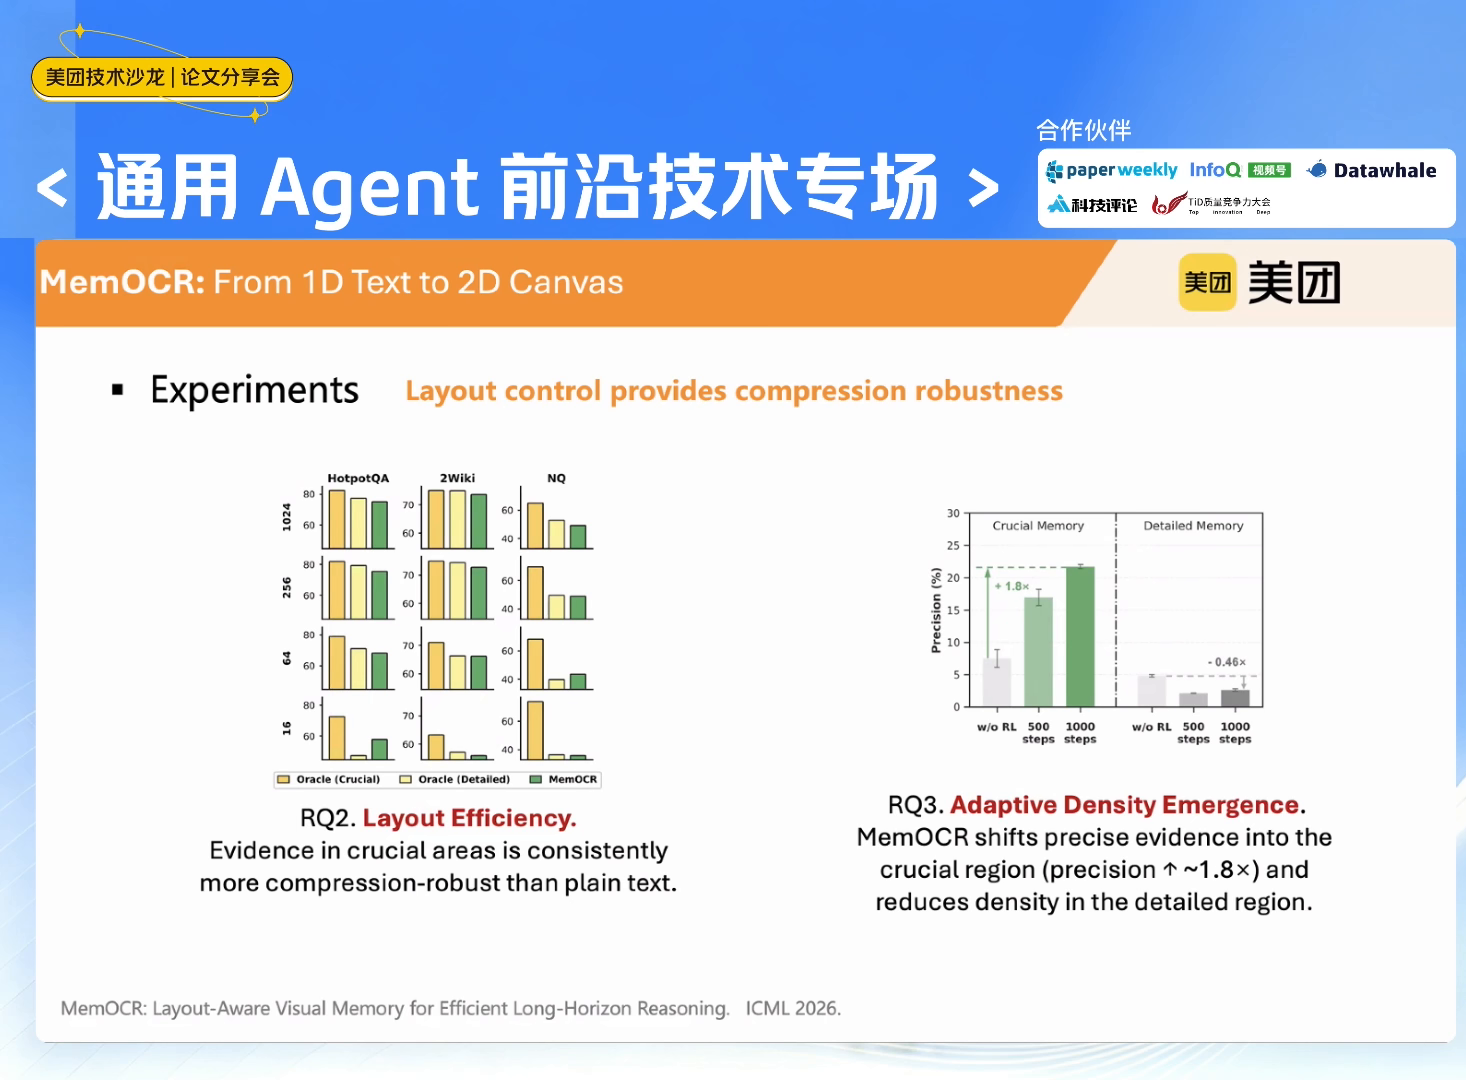
\includegraphics[width=0.86\linewidth,height=0.40\textheight,keepaspectratio]{figures/selected/frame_0032_layout_efficiency_density_emergence.png}
\caption{Layout efficiency 与证据区域：左侧柱状图对比 oracle 证据位于 crucial area 与 detail area 时的效果，显示关键区域中的证据更抗压缩；右侧图展示训练后关键证据更倾向进入 crucial area。\protect\footnotemark}
\end{figure}
\footnotetext{视频画面时间区间：00:15:30--00:16:00。}

这里需要小心解释 oracle analysis。它不是部署时可用的作弊机制；它是诊断工具，作用类似给系统做“定位实验”。如果正确答案放在高显著区域后效果明显变好，就说明模型确实受益于位置和显著性。如果正确答案放在低显著区域后收益有限，甚至让结果变差，就说明低显著区域在强压缩下可读性不足，继续往里面塞答案会增加视觉负担。

\begin{warningbox}{oracle 注入的反直觉风险}
把正确答案放进记忆并不自动提高性能。若答案被放进低效、拥挤、低显著的区域，它可能让局部文字更密，进一步降低可读性。视觉记忆的核心约束是“读得出”，单纯“写进去”没有保证。
\end{warningbox}

\subsection{从结果反推机制：layout control 是压缩率分配器}

主实验和 oracle analysis 合在一起，给出了一条机制链：

\begin{itemize}
    \item 长上下文问答需要在最终回答时恢复关键证据。
    \item \texttt{memory budget} 缩小时，低显著细节最先变得难读。
    \item \texttt{layout control} 让模型把答案相关证据放到高显著区域。
    \item 高显著区域在压缩后仍更可能被视觉语言模型识别。
    \item 因此 MemOCR 在极低预算下保留了更高的性能。
\end{itemize}

可以把 \texttt{layout control} 看成一种压缩率分配器。传统文本压缩像把所有文字统一缩小，标题、证据、边角细节一起变小；MemOCR 更像排版一张考试速查卡，把公式写在正中央，把条件放在旁边，把低频背景放在角落。容量同样有限，差别在于它承认信息价值不同，并让高价值信息占据更可靠的视觉通道。

这也解释了为什么视觉记忆的优势在极低预算下更明显。预算充足时，多数方法都还能保留不少信息；预算紧张时，系统必须做取舍。MemOCR 的训练目标让这种取舍变成可学习行为，实验结果说明这种行为确实转化成了问答鲁棒性。

\subsection{本章小结}

本章的核心信息可以压缩成三句话。第一，MemOCR 在长上下文单跳和多跳问答中整体优于文本记忆基线。第二，优势随着 \texttt{memory budget} 下降而更明显，字幕给出的关键数字是 $16$ 个视觉记忆 token 下仍保留 $80\%+$ 的完整上下文能力，而部分文本基线在极端预算下平均掉点约 $50\%--60\%$。第三，oracle analysis 说明性能来源与 \texttt{layout control} 直接相关：同一条正确证据放在 \texttt{crucial area} 比放在 \texttt{detail area} 更有价值。

这一章同时暴露了后续章节要继续追问的问题：模型是否真的学会了把关键证据主动放进高显著区域；这种视觉记忆策略的额外成本是否值得；如果视觉记忆写得过密或比较关系被低估，系统会怎样失败。随后的学习行为、成本与失败模式章节将依次回答这三个问题。
